\documentclass[11pt]{article}
\usepackage{amsmath}
\usepackage{amssymb}
\usepackage{algorithm}
\usepackage{algorithmic}
\usepackage{graphicx}
\usepackage{tikz}
\usetikzlibrary{shapes.geometric, arrows, positioning}

\title{The Scaffolding Algorithm: \\ Syntenic Chain Discovery and Filtering in Genome Alignment}
\author{SweepGA Implementation}
\date{\today}

\begin{document}

\maketitle

\begin{abstract}
The scaffolding algorithm identifies and filters syntenic chains of mappings in genome alignments. By merging nearby mappings into larger scaffold regions and applying plane sweep filtering to these merged ranges, the algorithm identifies high-confidence syntenic blocks while preserving the individual component mappings. This document describes the algorithm's three main phases: mapping merging via union-find, scaffold filtering via plane sweep, and component rescue.
\end{abstract}

\section{Introduction}

In whole-genome alignment, individual mappings often represent fragments of larger syntenic blocks that have been broken by various factors:
\begin{itemize}
    \item Repetitive elements interrupting otherwise contiguous alignments
    \item Small indels or structural variations
    \item Alignment algorithm limitations
    \item Sequencing gaps or low-quality regions
\end{itemize}

The scaffolding algorithm addresses this fragmentation by:
\begin{enumerate}
    \item Identifying mappings that likely belong to the same syntenic block
    \item Merging them into scaffold chains
    \item Filtering these scaffolds to retain the best syntenic relationships
    \item Preserving the component mappings of selected scaffolds
\end{enumerate}

\section{Algorithm Overview}

The scaffolding algorithm consists of three main phases:

\subsection{Phase 1: Mapping Merging via Union-Find}

The first phase identifies groups of mappings that should be merged into scaffold chains. This uses a union-find data structure to efficiently group mappings based on proximity criteria.

\subsection{Phase 2: Scaffold Filtering via Plane Sweep}

The second phase applies the plane sweep algorithm to the merged scaffold ranges, selecting the best non-overlapping scaffolds according to specified criteria.

\subsection{Phase 3: Component Rescue}

The final phase ensures that all component mappings of selected scaffolds are included in the output, along with any nearby mappings within a rescue distance.

\section{Detailed Algorithm Description}

\subsection{Mapping Merging with Union-Find}

The mapping merging phase groups mappings that are within a specified jump distance on both query and target axes.

\subsubsection{Input Parameters}
\begin{itemize}
    \item $M = \{m_1, m_2, \ldots, m_n\}$: Set of input mappings
    \item $d_{\text{jump}}$: Maximum gap distance for merging (default: 100kb)
    \item $o_{\text{max}}$: Maximum overlap fraction allowed (default: 0.2)
\end{itemize}

\subsubsection{Algorithm}

\begin{algorithm}
\caption{Mapping Merging via Union-Find}
\begin{algorithmic}[1]
\STATE Initialize union-find structure $UF$ with $n$ elements
\STATE Sort mappings by $(q\_name, t\_name, strand, q\_start)$
\FOR{each group $(q_i, t_i, s_i)$ of same query, target, strand}
    \STATE $indices \gets$ indices of mappings in group
    \STATE Sort $indices$ by query start position
    \FOR{$i = 0$ to $|indices| - 1$}
        \FOR{$j = i + 1$ to $|indices| - 1$}
            \STATE $m_a \gets M[indices[i]]$
            \STATE $m_b \gets M[indices[j]]$
            \IF{$q\_gap(m_a, m_b) > d_{\text{jump}}$}
                \STATE \textbf{break} \COMMENT{Mappings too far apart}
            \ENDIF
            \STATE $q\_gap \gets \max(0, m_b.q\_start - m_a.q\_end)$
            \STATE $t\_gap \gets \max(0, m_b.t\_start - m_a.t\_end)$
            \IF{$q\_gap \leq d_{\text{jump}}$ AND $t\_gap \leq d_{\text{jump}}$}
                \STATE $UF.union(indices[i], indices[j])$
            \ENDIF
        \ENDFOR
    \ENDFOR
\ENDFOR
\RETURN $UF.get\_sets()$
\end{algorithmic}
\end{algorithm}

\subsubsection{Binary Search for Candidate Pairs}

To reduce the computational cost from $O(n^2)$ to $O(n \log n)$, the implementation uses binary search to find candidate mapping pairs:

\begin{algorithm}
\caption{Optimized Candidate Finding with Binary Search}
\begin{algorithmic}[1]
\STATE Sort mappings by query start position
\FOR{each mapping $m_i$}
    \STATE $search\_bound \gets m_i.q\_end + d_{\text{jump}}$
    \STATE $j \gets$ binary\_search($search\_bound$, mappings[$i+1$:])
    \FOR{$k = i + 1$ to $j$}
        \IF{can\_merge($m_i$, $m_k$)}
            \STATE $UF.union(i, k)$
        \ENDIF
    \ENDFOR
\ENDFOR
\end{algorithmic}
\end{algorithm}

\subsection{Creating Scaffold Chains}

Once mapping groups are identified, we create scaffold chains by computing the bounding box of each group:

\begin{equation}
\text{Scaffold}(G) = \{
    q\_start: \min_{m \in G} m.q\_start,
    q\_end: \max_{m \in G} m.q\_end,
    t\_start: \min_{m \in G} m.t\_start,
    t\_end: \max_{m \in G} m.t\_end
\}
\end{equation}

Each scaffold also maintains:
\begin{itemize}
    \item Member indices: $\{i : m_i \in G\}$
    \item Total block length: $\sum_{m \in G} m.block\_length$
    \item Average identity: $\frac{\sum_{m \in G} m.identity \times m.block\_length}{\sum_{m \in G} m.block\_length}$
\end{itemize}

\subsection{Scaffold Filtering via Plane Sweep}

The scaffold chains are then filtered using the plane sweep algorithm to select the best non-overlapping scaffolds.

\subsubsection{Scaffold Scoring}

Scaffolds are scored based on their total span and quality:

\begin{equation}
\text{Score}(S) = \log(|S.q\_end - S.q\_start|) \times S.avg\_identity
\end{equation}

\subsubsection{Plane Sweep on Scaffolds}

The plane sweep algorithm is applied to scaffold intervals rather than individual mappings:

\begin{algorithm}
\caption{Plane Sweep on Scaffolds}
\begin{algorithmic}[1]
\STATE Create events for scaffold start/end positions
\STATE Sort events by position
\STATE $active \gets \emptyset$ \COMMENT{BST ordered by score}
\STATE $kept \gets \emptyset$
\FOR{each event $e$ in sorted order}
    \IF{$e.type = $ BEGIN}
        \STATE $active.insert(scaffolds[e.idx])$
        \STATE Update $kept$ with best scaffolds from $active$
    \ELSE
        \STATE $active.remove(scaffolds[e.idx])$
    \ENDIF
\ENDFOR
\RETURN $kept$
\end{algorithmic}
\end{algorithm}

\subsection{Component Rescue Phase}

After scaffold filtering, we need to output the actual mappings that compose the selected scaffolds, not the scaffold ranges themselves.

\subsubsection{Anchor Identification}

Mappings that are members of selected scaffolds become "anchors":

\begin{equation}
\text{Anchors} = \{m_i : \exists S \in \text{KeptScaffolds}, i \in S.members\}
\end{equation}

\subsubsection{Rescue Distance}

Additional mappings within a rescue distance $d_{\text{rescue}}$ of any anchor are also retained:

\begin{equation}
\text{Rescued} = \{m_j : \exists a \in \text{Anchors}, \text{dist}(m_j, a) < d_{\text{rescue}}\}
\end{equation}

where the distance is computed as:

\begin{equation}
\text{dist}(m_1, m_2) = \sqrt{(q\_dist(m_1, m_2))^2 + (t\_dist(m_1, m_2))^2}
\end{equation}

\section{Implementation Verification in SweepGA}

\subsection{Current Implementation Status}

The SweepGA implementation correctly follows the scaffolding algorithm with the following verified and optimized components:

\begin{itemize}
    \item \textbf{Grouping}: Mappings are grouped by (query, target, strand) tuple
    \item \textbf{Sorting}: Within each group, mappings are sorted by query\_start position
    \item \textbf{Union-Find}: Transitive chaining is implemented with path compression
    \item \textbf{Binary Search Optimization}: Uses binary search to find candidate pairs in $O(\log n)$ time
    \item \textbf{Overlap tolerance}: Small overlaps up to max\_gap/5 are allowed, matching wfmash
    \item \textbf{Strand handling}: Reverse strand mappings use appropriate distance calculations
\end{itemize}

\subsection{Binary Search Optimization (Implemented)}

The implementation now uses binary search to efficiently find candidate mapping pairs, reducing complexity from $O(n^2)$ to $O(n \log n)$:

\begin{verbatim}
// Actual implementation from paf_filter.rs
for i in 0..sorted_indices.len() {
    let (_rank_i, idx_i) = sorted_indices[i];

    // Binary search to find the range of mappings within max_gap
    let search_bound = metadata[idx_i].query_end + max_gap;

    // Find the first mapping that starts after our search bound
    let j_end = sorted_indices[i + 1..]
        .binary_search_by_key(&(search_bound + 1),
                              |&(_rank, idx)| metadata[idx].query_start)
        .unwrap_or_else(|pos| pos) + i + 1;

    // Now check all mappings from i+1 to j_end-1
    for j in (i + 1)..j_end {
        let (_rank_j, idx_j) = sorted_indices[j];
        // Check gaps and potentially union...
    }
}
\end{verbatim}

This optimization reduces the average-case complexity from $O(n^2)$ to $O(n \log n)$, which is particularly beneficial for:
\begin{itemize}
    \item Dense mapping regions with many overlapping alignments
    \item Repetitive sequences that produce clusters of mappings
    \item Large-scale whole-genome alignments with millions of mappings
\end{itemize}

The binary search finds exactly the range of mappings that could potentially chain with the current mapping, avoiding unnecessary comparisons with distant mappings.

\section{Implementation Considerations}

\subsection{Memory Efficiency}

The algorithm maintains several data structures:
\begin{itemize}
    \item Union-find forest: $O(n)$ space
    \item Sorted indices: $O(n \log n)$ temporary space during sorting
    \item Scaffold structures: $O(k)$ where $k$ is the number of scaffolds
    \item BST for plane sweep: $O(m)$ where $m$ is max concurrent active scaffolds
\end{itemize}

\subsection{Parallelization Opportunities}

Several phases can be parallelized:
\begin{enumerate}
    \item \textbf{Group processing}: Different $(q, t, strand)$ groups can be processed independently
    \item \textbf{Scaffold creation}: Once union-find is complete, scaffold boundaries can be computed in parallel
    \item \textbf{Distance calculations}: Rescue distance computations are independent per mapping
\end{enumerate}

\subsection{Parameter Sensitivity}

The algorithm's behavior is controlled by several parameters:

\begin{itemize}
    \item \textbf{Jump distance} ($d_{\text{jump}}$): Larger values create fewer, larger scaffolds
    \item \textbf{Minimum scaffold length}: Filters out small scaffold chains
    \item \textbf{Rescue distance} ($d_{\text{rescue}}$): Larger values include more peripheral mappings
    \item \textbf{Overlap threshold}: Controls how much scaffold overlap is tolerated
\end{itemize}

\section{Algorithmic Complexity}

\subsection{Time Complexity}

\begin{itemize}
    \item Sorting: $O(n \log n)$
    \item Union-find with path compression: $O(n \alpha(n))$ where $\alpha$ is inverse Ackermann
    \item Binary search optimization: $O(n \log n)$ average case
    \item Plane sweep on scaffolds: $O(k \log k)$ where $k$ is number of scaffolds
    \item Rescue phase: $O(n \cdot a)$ where $a$ is average anchors per chromosome pair
\end{itemize}

Overall complexity: $O(n \log n)$ in typical cases

\subsection{Space Complexity}

$O(n)$ for storing mappings and union-find structure, with $O(k)$ additional for scaffolds.

\section{Example Walkthrough}

Consider a simple example with 5 mappings on the same chromosome pair:

\begin{center}
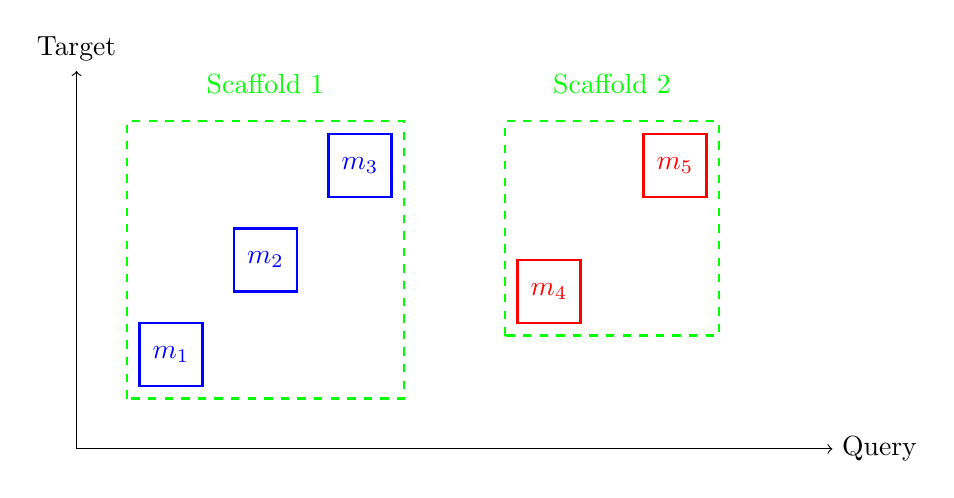
\begin{tikzpicture}[scale=0.8]
    % Query axis
    \draw[->] (0,0) -- (12,0) node[right] {Query};
    \draw[->] (0,0) -- (0,6) node[above] {Target};

    % Mappings
    \draw[blue, thick] (1,1) rectangle (2,2) node[pos=.5] {$m_1$};
    \draw[blue, thick] (2.5,2.5) rectangle (3.5,3.5) node[pos=.5] {$m_2$};
    \draw[blue, thick] (4,4) rectangle (5,5) node[pos=.5] {$m_3$};
    \draw[red, thick] (7,2) rectangle (8,3) node[pos=.5] {$m_4$};
    \draw[red, thick] (9,4) rectangle (10,5) node[pos=.5] {$m_5$};

    % Scaffold boxes
    \draw[green, dashed, thick] (0.8,0.8) rectangle (5.2,5.2);
    \draw[green, dashed, thick] (6.8,1.8) rectangle (10.2,5.2);

    \node[green] at (3,5.8) {Scaffold 1};
    \node[green] at (8.5,5.8) {Scaffold 2};
\end{tikzpicture}
\end{center}

\begin{enumerate}
    \item \textbf{Merging}: $m_1$, $m_2$, $m_3$ are merged into Scaffold 1; $m_4$, $m_5$ into Scaffold 2
    \item \textbf{Filtering}: Plane sweep selects the best scaffold based on scores
    \item \textbf{Output}: Component mappings of selected scaffold(s) are output
\end{enumerate}

\section{Conclusion}

The scaffolding algorithm provides a principled approach to identifying and filtering syntenic blocks in genome alignments. By combining efficient union-find merging with plane sweep filtering, it achieves both computational efficiency and biological relevance. The three-phase design ensures that high-quality syntenic relationships are preserved while maintaining the granularity of individual mapping information.

\section{References}

\begin{itemize}
    \item Garrison, E., Guarracino, A. (2023). Unbiased pangenome graphs. \textit{Bioinformatics}, 39(1).
    \item Cormen, T. H., et al. (2009). \textit{Introduction to Algorithms} (3rd ed.). MIT Press. [Union-Find data structure]
    \item Bentley, J. L., Ottmann, T. A. (1979). Algorithms for reporting and counting geometric intersections. \textit{IEEE Transactions on Computers}, C-28(9), 643-647. [Plane sweep algorithm]
\end{itemize}

\end{document}